\chapter{Optical pumping of an atom laser}
\label{OpticalPumping}
\graphicspath{{Figures/OpticalPumping/}{Figures/Common/}}

The results presented in this chapter have been published in~\citet{Robins:2008,Doring:2009}.

\section{Motivation}

The development of the continuous-wave optical laser was a significant advance over the first pulsed ruby laser. The continuous-wave optical laser opened up many applications. The atom laser is a very promising source for both precision measurement and fundamental physics.

The replenishment process can be divided into two critical components: a delivery system for filling an atomic reservoir with ultracold atoms and a pumping mechanism for irreversibly and continuously transferring atoms from the reservoir to the laser mode.

The technical requirements on both parts of the replenishment system are stringent. Nonetheless, recent experiments have demonstrated that a delivery system for atoms is feasible and possible.~\citet{Chikkatur:2002qa} showed that Bose-condensed atoms could be periodically transported over large distances using a moving optical dipole trap. Further experiments with transport, based on interference of two counter-propagating lasers, have shown that dipole trapping techniques could be extended to provide continuous delivery of atoms~\citep{Schmid:2006}. Magnetic guiding systems for ultracold atoms may also provide a path to future delivery systems~\citep{Lahaye:2004,Greiner:2001,Greiner:2007}.

The realisation of the pumping mechanism for a continuous atom laser has proved more problematic. There are four critical requirements that are difficult to satisfy experimentally. First, the atoms should enter the laser mode continuously and coherently, that is, with the phase and amplitude of the lasing condensate. Thus, atoms must make a transition that is Bose-stimulated by the atomic lasing mode. The second requirement is that the pumping process is irreversible. It requires coupling to a reservoir. There are two reservoirs available, the empty modes of the electromagnetic field accessible via a transition from an excited atomic state, or the empty modes of the atomic field accessible via evaporation. For a high-coherence atom laser, the lasing mode must be a pure condensate with a significantly smaller thermal fraction, making evaporation-induced pumping a difficult possibility for the production for a highly coherent continuous atom laser. The third requirement is that the pumping system must be compatible with a continuous replenishment mechanism. This suggests strongly that there be a physical separation between the source and the lasing condensates. A physical separation with a stimulated transition between the source and the lasing mode isolates the lasing mode from phase kicks and heating that would result either as a necessary consequence of the replenishment system (for example in the replenishment system demonstrated by~\citet{Chikkatur:2002qa} where condensates are merged) or as a consequence of an imperfect delivery system. Finally, the fourth condition on a pumping system is that it should be possible to continuously output-couple atoms from the laser mode into a beam, while the pumping mechanism is operating.

The two possibilities for reservoirs to supply the irreversibility necessary for the proper operation of a pumped atom laser (Bose-Einstein condensate) are considered in this chapter and the next. In this chapter, pumping an atom laser using interactions mediated by light is considered. In this case the reservoir providing the irreversibility are the vacuum electromagnetic modes into which light is scattered by the pumping process. \chapterref{KineticTheory} considers the alternate possibility of using atomic \emph{s}-wave scattering interactions to mediate the pumping process with evaporation to make the process irreversible.

\hrule

Previous work on light-BEC interactions. Rayleigh/Raman superradiance, EIT, CARL, and the rest of that list that I had.


\section{Pumping mechanism}
\label{OpticalPumping:PumpingMechanism}

\begin{figure}
    \centering
    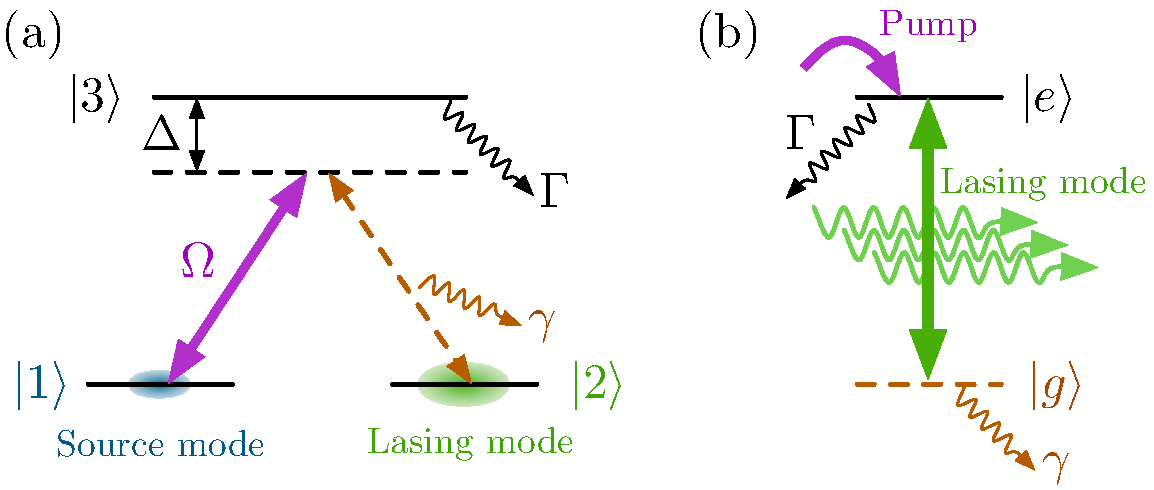
\includegraphics[width=14cm]{LambdaModel}
    \caption{FIXME: This is not a caption. Comparison of considered atom laser pumping scheme (a) and typical optical laser pumping scheme (b).\label{OpticalPumping:LambdaModel}}
\end{figure}

The optical pumping process under investigation in this chapter is illustrated in \figureref{OpticalPumping:LambdaModel}(a).  In this process atoms in the source mode are driven by a laser into an excited state from which they can decay into the lasing mode (the condensate).  Although there is no laser driving this second transition ($\ket{3}\leftrightarrow\ket{2}$), the decay of atoms into the lasing mode is not spontaneous emission in the usual sense.  The emission process is \emph{atomically}-stimulated by the large occupation of the lasing mode in the same way that the transition may be \emph{optically}-stimulated even in the absence of any population in the atomic state into which the atom decays.

The final decay of an atom into the lasing mode in \figureref{OpticalPumping:LambdaModel} resembles standard \emph{optical} laser schemes [see \figureref{OpticalPumping:LambdaModel}(b)] in which the roles of atoms and light are reversed.  In an optical laser an atom in the excited state is stimulated to emit into the ground state by the resonant photons in the laser cavity.  Once the atom has emitted, it decays rapidly into other internal states with rate $\gamma$ significantly limiting reabsorption from the $\ket{g}$ state.  A similar process occurs in the proposed optical pumping scheme in which the photon emitted as the atom decays  leaves the system rapidly preventing reabsorption.  The loss of photons from the system is represented by the decay of the optical mode with rate $\gamma$ in \figureref{OpticalPumping:LambdaModel}(a).

This similarity between the proposed atom laser pumping mechanism and the usual optical laser pumping mechanism is clearly illustrated by considering the Hamiltonian coupling the excited and ground atomic states in \figureref{OpticalPumping:LambdaModel}
\begin{align}
    \hat{H} &= \hbar \epsilon \left(\hat{a}_e^\dagger \hat{a}_g \hat{a}_\text{ph} + \hat{a}_g^\dagger \hat{a}_\text{ph}^\dagger \hat{a}_e  \right),
    \label{OpticalPumping:TwoLevelAtomHamiltonian}
\end{align}
where $\epsilon$ is a real coupling constant, the $\hat{a}_e$, $\hat{a}_g$, and $\hat{a}_\text{ph}$ are annihilation operators for the atomic excited state, atomic ground state and photon mode respectively.  The rotating wave approximation has been made in obtaining this Hamiltonian, assuming that the optical mode is not detuned from the atomic transition by a large fraction of the frequency difference between the two states.  

The Hamiltonian \eqref{OpticalPumping:TwoLevelAtomHamiltonian} describes both the atom- and optical-laser pumping mechanisms, the difference in the mechanisms being in the occupations of the various states.  If the system is initially in a state with $N_e$ atoms in the atomic excited state, $N_g$ atoms in the atomic ground state and $N_\text{ph}$ photons in the optical mode, the amplitude for an atom in the excited state to emit a photon is
\begin{align}
    \bra{N_e-1, N_g + 1, N_\text{ph} + 1} \hat{H} \ket{N_e, N_g, N_\text{ph}} &= \hbar \epsilon \sqrt{N_g+1} \sqrt{N_\text{ph}+1} \sqrt{N_e}.
\end{align}
This emission process can therefore be stimulated either by photons ($N_\text{ph} > 0$) or by atoms ($N_\text{g} > 0$).  It would also be possible for the emission to be stimulated by both photons \emph{and} atoms, although in this case the amplitude for the absorption process would be non-zero
\begin{align}
    \bra{N_e+1, N_g - 1, N_\text{ph} - 1} \hat{H} \ket{N_e, N_g, N_\text{ph}} &= \hbar \epsilon \sqrt{N_e+1} \sqrt{N_\text{ph}} \sqrt{N_g}.
\end{align}
It is for this reason that it is desirable in an optical laser to have $N_g \approx 0$, and in the proposed atom laser pumping scheme to have $N_\text{ph} \approx 0$.

Atom laser pumping schemes of the form of that illustrated in \figureref{OpticalPumping:LambdaModel}(a) have been proposed before~\citep{Olshanii:1996,Janicke:1996,Spreeuw:1995,Cirac:1996rr,Cirac:1996,Santos:2000,Castin:1998,Cirac:1994,Vengalattore:2003,Santos:2001ve,Wolf:2000,Santos:1999qf} for the production of BEC without the use of collisional evaporation and its consequent losses.  The main problem that they all seek to address is that of reabsorption of photons spontaneously emitted when the atom in state $\ket{3}$ decays to the $\ket{2}$ state, but not to the lasing mode.  This emitted photon will be resonant with the lasing mode and may be scattered several times before finally leaving the condensate.  A single such spontaneously emitted photon can cause significant heating of a condensate as the single photon recoil energy can be as large as or greater than the chemical potential of the condensate.

One proposed method~\citep{Castin:1998,Vengalattore:2003} for reducing the heating uses a purely geometric solution: if a condensate is made sufficiently narrow in one or more dimensions such that a photon emitted in one of those directions is negligibly likely to be reabsorbed, the overall probability for reabsorption will also be reduced.  While this method may be appropriate for the initial formation of BEC, it is impractical for a large BEC as the trap deformation necessary to reach the required regime is extreme.  For a \nucl{87}{}{Rb} condensate of $N= 5\times 10^5$ atoms with trapping frequencies of $\omega_x = \omega_y = \unit[2\pi \times 128]{Hz}$, $\omega_z = \unit[12.8]{Hz}$, the mean-free path in the centre of the condensate for a resonant photon on the cycling transition ($\lambda = \unit[780]{nm}$) is $1/(n \sigma) = \unit[16]{nm}$ where $n$ is the peak condensate density and $\sigma = 3 \lambda^2/2 \pi$ is the atomic scattering cross-section.

Another possibility for reducing reabsorption that works well in optical lattices is to operate in the \emph{festina lente} regime~\citep{Wolf:2000,Santos:1999qf,Cirac:1996,Castin:1998} in which the energy levels of the trap are sufficiently separated such that a photon emitted when an atom decays into a particular trap level is only resonant with atoms in that level (and those levels degenerate with it).  This prevents the occurrence of `dangerous' processes in which an excited atom decays into a non-condensate level with the emitted photon being absorbed by the condensate.  In the case of resonant optical pumping light ($\Delta = 0$ in \figureref{OpticalPumping:LambdaModel}(a)), the \emph{festina lente} regime requires that $\omega_\text{min} \gg \Gamma$  where $\omega_\text{min}$ is the minimum of the magnetic trapping frequencies.  Strictly, the \emph{festina lente} regime has only been investigated in the absence of \emph{s}-wave scattering interactions, however one would expect that in the presence of \emph{s}-wave scattering the trap frequency energy scale would simply be replaced by the energy of the relevant Bogoliubov excitation (refer to \sectionref{Peaks:ElementaryExcitations}).  Regardless, the \emph{festina lente} regime is impractical to achieve in alkali gases like \nucl{87}{}{Rb} as the relevant decay rate is $\Gamma = \unit[2\pi\times 5.9]{MHz}$, which is much larger than typical trap frequencies ($\omega \sim \unit[2\pi \times 100]{Hz}$) and condensate excitations ($\mu/\hbar \sim \unit[2\pi \times 10]{kHz}$).

A third possibility for reducing reabsorption is to operate in the \emph{boson accumulation regime} (BAR)~\citep{Cirac:1996rr,Floegel:2001} in which an atom in the excited state is significantly more likely to decay into the condensate mode than into all other modes.  In this limit it can be shown that absorption of emitted photons by atoms not in the condensate mode can be neglected.  It is in the BAR that we wish to operate our proposed pumping mechanism of \figureref{OpticalPumping:LambdaModel}(a).  

Up to this point, the source mode was entirely arbitrary; without consideration of reabsorption the proposed pumping process would work equally well for coherent or thermal states in the source mode.  As the optical transition between the excited atomic state and the lasing mode is not driven by a laser, the phase of the photons emitted is determined by the relative phase between the source and lasing modes; the direction of population transfer does not depend on the phase difference between these two modes. However the requirement that excited atoms be significantly more likely to decay into the condensate mode than to any other mode places a stringent requirement on the source mode of the pumping mechanism.  For this requirement to be satisfied, the momentum width of the source atom distribution cannot be significantly larger than the momentum width of the condensate.  If this were not the case a significant fraction of the atoms would not be momentum-resonant with the condensate under the pumping process and will therefore not be in the boson accumulation regime.  These atoms would be able to reabsorb spontaneously emitted photons causing the reabsorption problem previously discussed.  For an atomic distribution to have a momentum width comparable to that of the target condensate, the atoms must either be condensed or if they are thermal, be trapped in a significantly weaker trap than the target condensate mode and have a temperature below the condensation temperature in the tighter trap.  

Although it would be desirable to be able to use a thermal source of atoms as the source mode, the remainder of this chapter will investigate the possibility of using a coherent source of atoms as the source mode of the pumping mechanism.  Specifically, this coherent source will be an atom laser extracted from a second, source condensate.  Continuous operation of this scheme could in principle be achieved by replacing the source condensate with an independently-produced condensate once it is depleted.  As the pumping mechanism is independent of the phase-difference between the source and lasing modes this will not affect the direction of population transfer.

% \parasep
% 
% The pumping mechanism described in this section bears some resemblance to other optical processes that can occur in Bose-Einstein condensates such as EIT, and Rayleigh/Raman superradiance. FIXME: Complete paragraph/s.
% 
% Quote from the paper:
% 
% The mechanism we have described for pumping is related to pulsed Raman super-radiance that has been studied previously.  In our work, in the laboratory frame, atoms are driven from the $\ket{2, 0}$ untrapped state into the $\ket{1, -1}$ trapped state enabling us to continue pumping indefinitely.  the condensate that we pump is stationary in the laboratory frame.  Furthermore, our experiment is carried out in a double-condensate geometry with internal states that enable simultaneous pumping and outcoupling to produce a freely propagating atom laser beam from a simultaneously pumped condensate.
% 
% There is a second mechanism that we have considered that is related to the EIT mechanism described in the work by~\citet{Ginsberg:2007fk}.  Similar to the existing Raman super-radiance experiments, their work was necessarily carried out in a pulsed regime.  In our experiment, again, the geometry and choice of internal states enable the possibility of carrying out a related experiment continuously.  The condensates in such an experiment must have some spatial overlap.  The $\ket{2, 0}$ atoms are produced in the overlap region where the $\pi$-polarised pump beam is absorbed and the $\sigma$-polarised beam is produced.  Both beams travel in the same direction.  The amplitude of the $\pi$-polarised beam decays in the overlap region.  The amplitude of the $\sigma$-polarised beam grows.  The atoms follow the dark state and are pumped continuously to the lasing mode.


\section{The continuous pumping experiment}
\label{OpticalPumping:ContinuousExperiment}

A summary is provided here of the continuous pumping experiment performed by \emph{Nick Robins}, \emph{Cristina Figl} and \emph{Matthew Jeppesen} at the Department of Quantum Science, ANU.  Further details of the experimental setup and results are published in \citet{Robins:2008}.

\begin{figure}
    \centering
    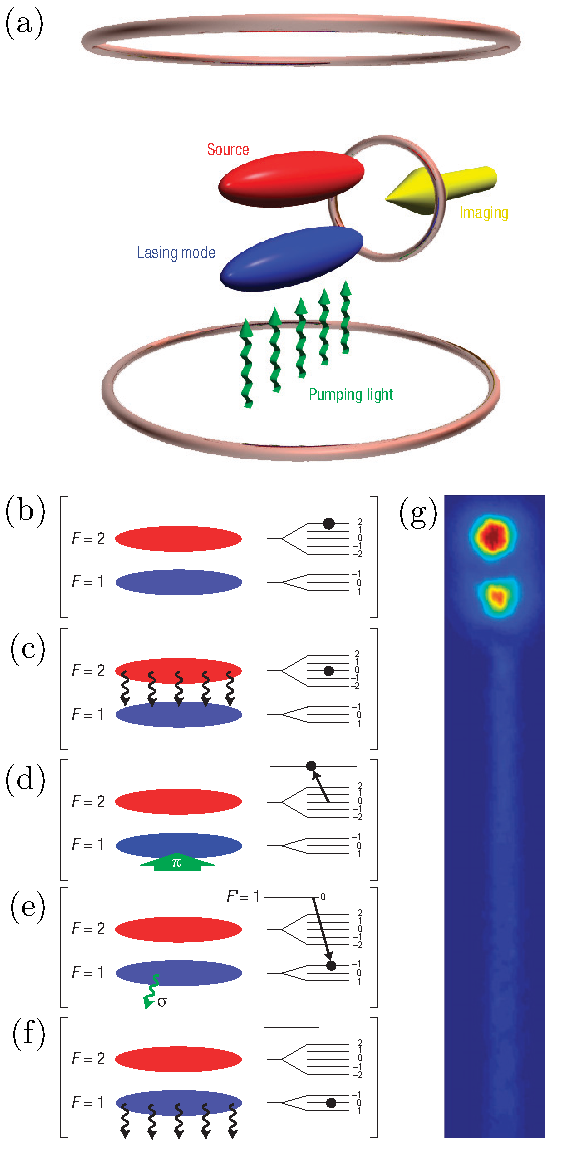
\includegraphics[width=8cm]{ExperimentSchematic}
    \caption{FIXME: Caption.  Schematic diagram of the operation of the pumped atom laser.  Schematic diagram of the experiment (a) and pumping steps (b--f).  A radiofrequency field spin-flips the atoms to the $\ket{2, 0}$ state (b), and they fall under gravity (c).  The light field couples the atoms to the $F'=1$ excited state from which they are stimulated to emit into the $\ket{1, -1}$ BEC.  The atomic momentum is cancelled by the absorption and emission of the photons (d, e).  A second radiofrequency field finally output-couples the atoms into the $\ket{1, 0}$ atom laser (f).  (g), Absorption image of the experimental system, showing source, laser mode and output beam.}
    \label{OpticalPumping:ExperimentSchematic}
\end{figure}

\begin{table}
    \centering
    \begin{tabular}{cc}
    \toprule
    Parameter & Value\\
    \midrule
    $\ket{F=2, m_F=2}$ (source) condensate number & $N_\text{source} = (6.7 \pm 0.5)\times 10^5$ \\
    $\ket{F=1, m_F=-1}$ (laser) condensate number & $N_\text{laser} = (5.0 \pm 0.4) \times 10^5$ \\
    Radial trapping frequency (for $\ket{1, -1}$) & $\omega_r = \unit[2\pi \times 130]{Hz}$ \\
    Axial trapping frequency (for $\ket{1, -1}$) & $\omega_z = \unit[2\pi \times 13]{Hz}$ \\
    \bottomrule
    \end{tabular}
    \caption{Experimental parameters for the Rubidium-87 BEC system under consideration.}
    \label{OpticalPumping:ExperimentalParameters}
\end{table}


To produce a pumped atom laser two independent condensates are prepared in the $\ket{F=2, m_F=2}$ and $\ket{F=1, m_F=-1}$ magnetically trapped states of \nucl{87}{}{Rb}.  Owing to their larger magnetic moment, the $\ket{2, 2}$ atoms are more tightly confined in the magnetic field than the $\ket{1, -1}$ atoms, and hence the evaporation does not directly cool them.  They are, however, sympathetically cooled through elastic collisions with the $\ket{1, -1}$ atoms~\citep{Myatt:1997}.  For the condensate numbers and trapping frequencies given in \tableref{OpticalPumping:ExperimentalParameters} the Thomas-Fermi radius of each cloud is approximately $\unit[5]{\micro m}$ in the vertical direction.  The different magnetic moments of the two clouds lead to a gravitational sag between their centres of $\unit[8]{\micro m}$. Hence, the two clouds of atoms overlap only slightly, with the $\ket{2, 2}$ source condensate located above the $\ket{1, -1}$ laser-mode condensate [see \figureref{OpticalPumping:ExperimentSchematic}(a)].

To measure the effect of pumping, it is essential that the number of atoms in each state is stable from one experimental run to the next.  For this purpose, many details of the apparatus were refined, including very efficient baffling against stray resonant light, very low uncertainty and drift in laser frequency, intensity and polarisation, and good vibrational and thermal stability of the trap.  The stability of the number of atoms in each state was determined for a data set comprising 20 measurements, and found to be as low as 1\%.

The operation of the experiment is illustrated in \figureref{OpticalPumping:ExperimentSchematic}.  Starting with an initial number of atoms in each state [\figureref{OpticalPumping:ExperimentSchematic}(b)], a weak continuous radiofrequency field is applied to the upper source cloud which couples atoms from the $\ket{2, 2}$ state, through $\ket{2, 1}$ to the $\ket{2, 0}$ state.  This coupling is highly spatially selective and does not affect the $\ket{1, -1}$ cloud.  These atoms begin to fall away from the $\ket{2, 2}$ source cloud [\figureref{OpticalPumping:ExperimentSchematic}(c)].  Simultaneously approximately $\unit[10]{pW}$ of upward propagating $\pi$-polarised light resonant with the $\ket{F=2}\rightarrow\ket{F'=1}$ transition is applied.  Although this light is resonant in energy with the $\ket{2, 2}$ source atoms, they are prevented from absorbing photons by atomic selection rules.  Hence, the source cloud is unaffected by the pumping light.  For pumping the laser mode, the $\ket{2, 0}$ atoms will absorb the pumping light [\figureref{OpticalPumping:ExperimentSchematic}(d)].  As these atoms fall, they may make a transition into the excited $\ket{F'=1, m_F=0}$ state from which they are stimulated to emit into the laser mode $\ket{1, -1}$ by the atoms already present in that mode [\figureref{OpticalPumping:ExperimentSchematic}(e)].  The $\sigma^{+}$-photon emitted in this process carries the phase difference between the pump atoms and the condensate.  Finally, the $\ket{1, -1}$ laser-mode atoms are output-coupled to produce the atom laser beam in the $\ket{1, 0}$ state [\figureref{OpticalPumping:ExperimentSchematic}(f)].  An absorption image of the ultracold atoms used to build the pumped atom laser system is shown in \figureref{OpticalPumping:ExperimentSchematic}(g).

For successful pumping, the pump atoms must be momentum-resonant with the lasing condensate.  This means that their atomic velocity after the emission of the photon has to lie within the velocity spread of the BEC.  The magnetic trapping frequencies were chosen not only to position the two clouds as closely as possible without significant overlap, but also such that the velocity acquired by a $\ket{2, 0}$ atom in falling from the centre of the $\ket{2, 2}$ cloud to the centre of the $\ket{1, -1}$ laser mode ($\unit[12]{mm\, s\textsuperscript{-1}}$) can be cancelled by the absorption of an appropriately directed and phased $\sigma^{+}$-photon; a single-photon recoil corresponds to $\unit[6]{mm\, s\textsuperscript{-1}}$.  The velocity at the laser-mode centre can be tuned by around $\unit[\pm 2]{mm\, s\textsuperscript{-1}}$ by moving the coupling surface within the source cloud up or down.  While the pump atoms are falling through the $\ket{1, -1}$ laser mode, the velocity varies by $\unit[\pm 3]{mm\, s\textsuperscript{-1}}$ owing to gravity and the time for which the pumping atoms satisfy momentum resonance with the laser mode is much shorter ($\sim \unit[100]{\micro s}$) than the traversal time across the laser mode ($\sim\unit[1]{ms}$).  The velocity spread of the laser mode is of the order of $\unit[0.3]{mm\, s\textsuperscript{-1}}$; thus, cancelling the atomic momentum of the $\ket{2, 0}$ state requires an extreme level of control over pumping parameters.  In the experiment no collective motion, such as sloshing or breathing of either the source- or laser-mode condensates was observed.  This implies that if excitations driven by the pumping exist, they occur with an amplitude of less than 5\% of the full-width at half-maximum of the laser-mode condensate, which was inferred from the resolution limit of the imaging system.

\begin{figure}
    \centering
    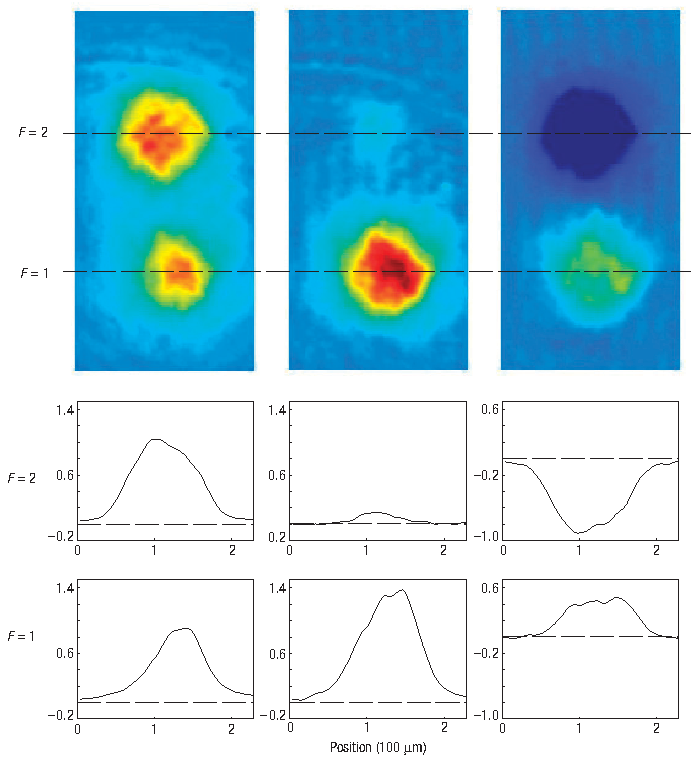
\includegraphics[width=12cm]{ExperimentalResults}
    \caption{FIXME: Caption.  Blue-detuned absorption images averaged over three identical runs of the experiment (top row); detuning of the probe laser from resonance is $\unit[7]{MHz}$.  The graphs below are horizontal cross-sections through the absorption images, showing optical depth, averaged over $\unit[50]{\micro m}$ in the vertical direction.  The tree columns correspond to: pumping off (left); pumping on (centre); difference between pumped and unpumped (right).}
    \label{OpticalPumping:ExperimentalResults}
\end{figure}

To isolate and study the pumping mechanism, the experiment was first operated without outcoupling from the laser-mode condensate.  \figureref{OpticalPumping:ExperimentalResults} demonstrates the effect \unit[200]{ms} of pumping has on the $\ket{1, -1}$ condensate; the left-hand image is taken without outcoupling from either condensate and without the pumping light.  The absorption image shows the unpumped $F=1$ laser-mode BEC (the lower cloud) with the $F=2$ source atoms above.  The curves below are horizontal cross-sections through the absorption images showing the optical depth of each atom cloud.  The central image shows the effect of \unit[200]{ms} of pumping on the laser-mode BEC.   The source is almost completely depleted and the laser-mode atom number has increased to $(7.2 \pm 0.4)\times 10^5$.  The third column shows the difference between the pumped and unpumped images. It is important to note that the profile of the laser-mode condensate after pumping has a significant Thomas-Fermi component with a small increase in the Gaussian thermal component.  The pumping efficiency, which is defined as the growth of the laser mode compared with the loss from the source, is $(35 \pm 10)\%$ for the results presented in \figureref{OpticalPumping:ExperimentalResults}.

A second experiment was also performed simultaneously pumping the laser-mode BEC and outcoupling from this condensate to demonstrate that the production of the atom laser could be operated independently of the pumping mechanism into the condensate.  In this chapter we focus on the results of the first experiment in which the pumping mechanism was studied.

\parasep

The continuous pumping experiment just described was designed to transfer $2 \hbar k$ of momentum to the falling pump atoms (by absorbing a photon of momentum $\hbar k$ going up and then emitting a photon of similar momentum directed downwards) as they are transferred to the laser-mode condensate.  However, there is a second way for the pump atoms to be momentum-resonant with the laser-mode condensate.  If the outcoupling surface for the upper condensate is towards the lower edge of the condensate the outcoupled atoms will be in close proximity to the laser-mode condensate immediately below due to the slight spatial overlap.  These recently outcoupled atoms will have almost no momentum and will be able to absorb a $\pi$-polarised photon with momentum $\hbar k$ upwards and emit a $\sigma^+$-polarised photon of similar momentum also directed upwards, decaying into the lower laser-mode condensate with no net momentum transfer.

These two different processes are examined in greater detail theoretically in \sectionref{OpticalPumping:MultimodeModel}, however we begin our theoretical analysis of the experiment and the pumping mechanism more generally with a simple single-mode model of the process illustrated in \figureref{OpticalPumping:LambdaModel}(a).


\section{Simple single-mode model}
\label{OpticalPumping:SingleModeModel}

We begin our theoretical investigation of the pumping mechanism behind the previously-described experiment by considering the simplest-possible model, a single-mode mean-field approximation to the process illustrated in \figureref{OpticalPumping:LambdaModel}(a).  The equations of motion for this model are
\begin{subequations}
    \label{OpticalPumping:SingleModeModel}
    \begin{align}
        \frac{d}{dt} c_\text{source} &= -i \Omega^* c_\text{excited} \\
        \frac{d }{dt}c_\text{excited} &= -i \Omega c_\text{source} -i g \alpha c_\text{lasing} - i \Delta c_\text{excited} - \frac{\Gamma}{2} c_\text{excited}\\
        \frac{d }{dt}c_\text{lasing} &= -i g^* \alpha^* c_\text{excited} \\
        \frac{d }{dt}\alpha &= -i g^* c_\text{lasing}^* c_\text{excited} - \frac{\gamma}{2} \alpha,
    \end{align} 
\end{subequations}
where $c_\text{source}$, $c_\text{lasing}$ and $c_\text{excited}$ are the amplitudes of the source $\ket{1}$, lasing $\ket{2}$ and excited $\ket{3}$ modes respectively, $\Omega$ is the complex Rabi frequency due to the pumping laser coupling the source and excited modes with detuning $\Delta$, $\alpha$ is the amplitude of the optical mode into which the excited atoms emit when decaying into the lasing mode and $g$ is the complex coupling constant for this transition.  The optical mode $\alpha$ will decay as photons propagate away from the system.  This process is modelled phenomenologically with a loss rate $\gamma$ from the optical mode $\alpha$.  The spontaneous decay of the excited state into modes other than the lasing mode occurs at a rate $\Gamma$.  It has been assumed that the pumping laser is sufficiently strong to be negligibly absorbed.  This assumption is relaxed in \sectionref{OpticalPumping:MultimodeModel}.  The evolution equations \eqref{OpticalPumping:SingleModeModel} are given in a rotating frame in which the energy difference between the source, excited and lasing modes have been appropriately removed.

In deriving \eqref{OpticalPumping:SingleModeModel} it has been assumed that atoms that undergo spontaneous decay from the excited mode will have no further impact upon the system.  In particular this means that the absorption of photons in the $\alpha$ mode by atoms in modes other than the lasing mode has been neglected.  The absorption of these photons by the lasing mode is, however, retained.  As discussed in \sectionref{OpticalPumping:PumpingMechanism} this is a valid approximation in the boson accumulation regime in which an excited atom is significantly more likely to decay into lasing mode than into any other mode.

The long-term dynamics of \eqref{OpticalPumping:SingleModeModel} will determine the usefulness of the process as a pumping mechanism.  The fast-timescale behaviour of this system can therefore be eliminated.  By far the fastest process in the system is the decay of the photons in the $\alpha$ mode as they leave the system.  The time taken for a photon to cross the width of a typical condensate ($\sim\unit[10]{\micro m}$) is $\sim\unit[10^{-13}]{s}$, giving $\gamma \sim \unit[10^{13}]{s\textsuperscript{-1}}$.  By comparison, the spontaneous decay rate of the excited mode is $\Gamma \sim \unit[10^8]{s\textsuperscript{-1}}$ for the $F'=1$ manifold of \nucl{87}{}{Rb}.  As the $\alpha$ mode reaches a quasistationary value on the fastest timescale in the system ($\gamma$), it can be adiabatically eliminated and replaced with its quasistationary limit,
\begin{align}
    \alpha & \approx -\frac{2 i g^*}{\gamma} c_\text{lasing}^* c_\text{excited}. \label{OpticalPumping:Alpha}
\end{align}

We next assume that the pump laser is driving the atoms in the weak-field regime, $\Omega \ll \max\left(\Delta, \Gamma\right)$.  In this limit, the excited mode $c_\text{excited}$ evolves on a more rapid timescale than either the source or lasing modes.  The excited mode may therefore also be adiabatically eliminated and replaced with its long-term average
\begin{align}
    c_\text{excited} &\approx \frac{-i \Omega c_\text{source}}{\frac{1}{2}\Gamma + 2 \frac{\abs{g}^2}{\gamma} N_\text{lasing} + i \Delta}, \label{OpticalPumping:CExcited}
\end{align}
where $N_\text{lasing} = \abs{c_\text{lasing}}^2$ is the number of atoms in the lasing mode.

With these two adiabatic eliminations made, the rate equations for the populations of the remaining two modes are obtained by substituting \eqref{OpticalPumping:Alpha} and \eqref{OpticalPumping:CExcited} into \eqref{OpticalPumping:SingleModeModel} giving
\begin{subequations}
    \label{OpticalPumping:SingleModeRateEquations}
    \begin{align}
        \frac{d}{dt} N_\text{source} &= - \frac{\abs{\Omega}^2 \left(\Gamma + \Gamma'\right)}{\abs{\frac{1}{2}(\Gamma + \Gamma') + i \Delta}^2} N_\text{source}\\
        \frac{d}{dt} N_\text{lasing} &= \frac{\Gamma'}{\Gamma + \Gamma'} \left( - \frac{d}{dt} N_\text{source}\right),
    \end{align}
\end{subequations}
where $\displaystyle \Gamma' = 4 \frac{\abs{g}^2}{\gamma} N_\text{lasing}$ is the rate constant with which atoms in the excited mode decay into the lasing mode.

The efficiency of the transfer of atoms in the pumping process is $\Gamma'/(\Gamma + \Gamma')$, which behaves as expected: as the occupation of the lasing mode $N_\text{lasing}$ is increased, the efficiency increases due to bosonic stimulation.  What is perhaps not expected is the behaviour of the transfer \emph{rate}.  In the limit of large detuning, $\Delta \gg \Gamma + \Gamma'$, the rate of atom transfer is
\begin{align}
    -\frac{d}{dt} N_\text{source} &\approx \frac{\abs{\Omega}^2}{\Delta^2} \left(\Gamma + \Gamma'\right) N_\text{source},
\end{align}
which increases as the lasing mode population increases (due to increasing $\Gamma'$).  In the limit of small detuning however ($\Delta \ll \Gamma + \Gamma'$) very different behaviour is obtained
\begin{align}
    -\frac{d}{dt} N_\text{source} &\approx 4 \frac{\abs{\Omega}^2}{\Gamma + \Gamma'} N_\text{source}, \label{OpticalPumping:SingleModePumpingRateZeroDetuning}
\end{align}
which \emph{decreases} as the lasing mode population increases.  This behaviour is due to the depletion of the excited state as $\Gamma'$ increases.  In the limit of small detuning, spontaneous and stimulated decay are the fastest processes reducing the occupation of the excited state, hence increasing those rates will reduce the overall population of the excited state.  In this limit as the excited state population decreases proportional to the square of these rates
\begin{align}
    N_\text{excited} &\approx 4 \frac{\abs{\Omega}^2}{(\Gamma + \Gamma')^2} N_\text{source},
\end{align}
the overall rate of atom transfer is suppressed as these processes occur on faster timescales.  In the opposite limit of large detuning, the spontaneous and stimulated decay processes are a perturbation on the Rabi-flopping process which populates the excited state.  In this limit the excited state population is independent of the spontaneous and stimulated emission rates
\begin{align}
    N_\text{excited} &\approx \frac{\abs{\Omega}^2}{\Delta^2} N_\text{source},
\end{align}
and the overall atom transfer rate into the lasing mode can be Bose-enhanced.

\parasep

The simple model developed in this section can be applied to the continuous pumping experiment described in \sectionref{OpticalPumping:ContinuousExperiment} to give a limit for the efficiency of the `$2 \hbar k$' momentum-transfer process.  In this process falling atoms outcoupled from the upper condensate reach a momentum of $2\hbar k$ vertically downwards before absorbing a pump photon of momentum $\hbar k$ from below and emitting a photon of similar momentum directed downwards to decay into the lasing mode.  If it is assumed that the intensity of the pump mode is approximately constant throughout the system, then the rate of transfer of atoms into the lasing mode cannot be faster than the rate of spontaneous emission while the source atoms are not momentum-resonant with the lasing mode\footnote{When the source atoms are not momentum-resonant with the lasing mode, it is equivalent to their being no photons in the lasing mode.  In this case, $\Gamma'=0$ and from \eqref{OpticalPumping:SingleModePumpingRateZeroDetuning} it can be seen that the spontaneous emission rate must be greater than the transfer rate into the condensate.}.  An upper bound for the efficiency of the `$2 \hbar k$' momentum-transfer process should therefore be given by the ratio of the time for which the source atoms are momentum-resonant with the condensate ($\sim\unit[100]{\micro s}$, see \sectionref{OpticalPumping:ContinuousExperiment}) to the fall time for the atoms to that point ($\sim\unit[1]{ms}$).  As the upper bound for this process $\sim 10\%$ is lower than the observed efficiency $\sim 35\%$, either the transfer of atoms into the lasing mode must significantly reduce the intensity of the pump mode, or it must be the `$0 \hbar k$' process that operates in the continuous pumping experiment.  The argument used to obtain an upper bound for the efficiency of the `$2 \hbar k$' momentum-transfer process does not apply to the `$0 \hbar k$' momentum-transfer process in which atoms outcoupled from the upper condensate can be immediately pumped into the lower condensate.

The simple model considered in this section does not take into account the behaviour of the emitted photons in the $\alpha$ mode as they traverse the source and/or lasing modes as they leave the system.  The investigation of this and other multimode effects is the subject of the next section and will be shown to lead to modifications of the behaviour described by the simple single-mode model.

\section{Multimode model (in 1D)}
\label{OpticalPumping:MultimodeModel}

The 1D model is based on the Maxwell-Schrödinger equations.  One of the technical difficulties is the fact that we must be able to solve in the case that light is travelling in opposite directions simultaneously.  It is not an issue analytically, the equations are well-defined.  The trouble is solving the system self-consistently.  The equations as posed are stiff and are best treated by implicit algorithms, but the best we have are half-arsed semi-implicit algorithms. Better yet would be to use a finite-element method and treat the cross-propagation properly, but I'm lazy.  The other issue is that the frequency of the light is usually known \emph{a priori}.  That is not the case for at least one of the modes in this system.  We therefore need to use some fancy tricks in order to get around that issue.  However, any detunings should not be too large.

Apart from the Maxwell part of the system of equations, everything else is fairly standard.  Except of course for the 1D reduction itself.  We'll call it a `central-line' approximation.

Somewhere in here we need to mention the adiabatic elimination and what kinds of terms it gives rise to.  And in what limit the approximation is valid (even close to resonance).

We need to talk about the other assumptions made in the model.  The assumption that spontaneous emission is negligible.  There is a question about how the 1D approximation affects the Franck-Condon factor, and the relationship between that and spontaneous emission.

Now is a good time to consider $0 \hbar k$ vs $2 \hbar k$ and resonant vs detuned in a simplified model in which things can be controlled (two overlapping modes in the same trap and where $k \rightarrow 0$). The important difference being the \emph{geometry}.

\subsection{3-level model}

This is a simplified model that contains only a small number of levels so that it is easier to keep track of what is going on.  We assume that we can outcouple directly from the $F=2$, $m_F=2$ trapped condensate to the $F=2$, $m_F=0$ state. This isn't realistic, but it is useful to simplify the whole process.  I believe the excited $F'$ manifold was also reduced.  With this simplified model we can investigate resonance vs detuned.  I seem to recall some crazy interesting physics where we had atom transfer back to the \emph{source} condensate in the $0 \hbar k$ configuration in the detuned case.  I believe it was all about phase differences and stuff.  If you look at the equations from the zero-dimensional model, the direction of transfer depends on the phase of a couple of terms, so it can go either way.  For the resonant case, the atoms were definitely transferred to the \emph{target} condensate, as desired.  Also, try as we might, it was not possible to get the $2 \hbar k$ resonance working efficiently.  Too much loss on the way.  Though I don't remember what happened in the detuned $2 \hbar k$ case.

This simplified 1D model contains all of the important physics related to the pumping process.  The delivery of atoms to the target condensate is simplified, and some of the optical transitions are removed.  This model is partly to validate the simple zero-dimensional model including some multimode dynamics, and also to try to get some basic agreement with the experiment before moving on to a more complete description in a later section.

\subsubsection{Comparison with experiment}

We consider both the $0\hbar k$ and the $2\hbar k$ resonance and find that we are able to get reasonable agreement with the experiment in the $0\hbar k$ limit, although it was incredibly fiddly to maximise the transfer.  The $2\hbar k$ resonance was dominated by loss of atoms as they travelled between the source and target condensates.  Although it must be stated that the experimentalists had a good idea of their detunings from rf spectroscopy.  The detunings did indicate that the required conditions for the $0 \hbar k$ resonance were not present.  They were however appropriate for the $2 \hbar k$ resonance, which was the one originally hoped for.  I can't remember, but I wanted to reproduce the experimental rf-spectroscopy data theoretically for some reason.

Anyway, things look great. So why don't we add more realism and see what we get? Maybe we can get even better agreement!

\subsection{5-level model}

The 5-level model is like the 3-level model, but including the full $F=2$ manifold.  Also, the full $F'=1$, $F'=2$ and $F'=3$ excited state manifolds are included before adiabatic elimination.  This model is designed to illustrate the full physics of the situation.  

\subsubsection{Comparison with experiment}

The theory in this case is completely defeated by the crazy mode shape of the $F=2$, $m_F=1$ level.  As this mode is trapped, it oscillates about the lower condensate.  If the intensity of the light is too low, these atoms block the pumping light from even reaching the target condensate and the $F=2$, $m_F=0$ atoms.  If the intensity of the light is too high, the atoms undergo spontaneous emission before they even reach the lower condensate, and you don't get any $F=2$, $m_F=0$ atoms.  If you try for something in the middle, the Franck-Condon factor between the $F=2$, $m_F=0$ atoms and the condensate is very small due to the crazy mode shape of the $F=2$, $m_F=1$ atoms from which the $F=2$, $m_F=0$ atoms are outcoupled.

In short, the 5-level model shows no pumping at all. But not because of something fundamental with the atom transfer process, but rather due to boring technical details about providing the atoms in the appropriate state and mode.  Besides, 1D models are very poor approximations to 5-level systems on timescales beyond the time for the $F=2$, $m_F=1$ atoms to reach the centre of that trap as the atoms will focus at the origin in the tight trapping dimension significantly increasing the density there over what would be seen in a purely 1D model.

\subsection{The pulsed pumping experiment}

The pulsed pumping experiment had the same basic set up as the continuous experiment, but instead a pulse of atoms (the \emph{transfer pulse}) was outcoupled from the upper condensate.  As this pulse was outcoupled over $\unit[100]{\micro s}$ (or whatever time it was) the issue of detuning essentially doesn't arise.  The Fourier width of the outcoupling pulse is large enough to essentially outcouple a copy of the condensate into the different Zeeman levels.  This transfer pulse was allowed to fall a variable delay time before pulsing on the same pumping light used in the continuous experiment.  The transfer pulse was finally allowed to fall further before imaging to determine the number of atoms remaining in the transfer pulse.  Due to the vastly different densities of the condensate and the transfer pulse, it is impossible to simultaneously measure the size of each.  Moreover, as the transfer pulse is significantly smaller than the target condensate, it was impossible to determine the number of transferred atoms to the target condensate.

\subsubsection{Theory / Experiment comparison}

We have good agreement with the loss of atoms out of the transfer pulse, which suggests that the $2 \hbar k$ resonance is workable, although it must be realised that operating a pulsed experiment is fundamentally different to the operation of the continuous experiment.  One model for the operation of the continuous experiment suggests that a process like STIRAP is occurring in the spatial domain instead of the usual temporal domain.  By operating the experiment in the pulsed regime, we are able to cause this process to occur in the temporal domain again, allowing access to the $2 \hbar k$ resonance.  Regardless, there are some questions that remain unanswered.  While we have good agreement on the transfer of atoms \emph{out} of the pulse, the experiment has no information about the transfer of atoms \emph{into} the condensate.  For this question, we can only rely on the theory.  In this case, the theory suggests that there should be a significant number of photons emitted spontaneously within the lower condensate.  A single one of these photons should cause significant (observable) heating of the lower condensate.  The issue is that no such heating is observed.  We are left scratching our heads on this issue (see next section).

\section{Discussion / Outlook}

This is where we say that we have reasonable evidence to say that we know what is going on in the transfer of atoms to the lower condensate, but a pretty poor explanation for what happens afterwards.  It is precisely this latter process that was thought to prevent optical pumping of condensates, and so the fact that the expected heating has not been observed is of great interest.  We can speculate wildly as to the origin of this absent heating, including BAR and quantum-mechanical collective effects due to the coherence of the atom laser.  Fundamentally, it seems to me that the notion of spontaneous emission is broken when the emission is occurring in the centre of a BEC.  On the edge, it probably mostly works.  In the centre, I'm not entirely convinced.

\section{Conclusion}

The conclusion I have been thinking of at the moment is along the following lines.  There have been three parts to the optical pumping process: (i) the delivery of atoms in an appropriate state to the condensate being pumped; (ii) the transfer of those atoms to the condensate being pumped; and (iii) the behaviour of the emitted photons within the pumped condensate.  This present chapter has aimed to understand part (ii) of this process.  Ideally we would also like to understand (iii) as it appears that there is some very interesting physics occurring in this part of the process, however we have fallen short of this goal.  By contrast process (i) is a technical detail of getting atoms to the lower condensate with an appropriate mode.  There are several methods that could be used for this process, and there are a number of arguments why the models used in this chapter are unsuitable for fully describing process (i).  Technical details are of course important, but not of fundamental importance.  And it has been the fundamentally important processes that we have aimed to investigate in the present chapter.
